  \documentclass[a4paper]{article}
\usepackage{amsmath}
\usepackage{amsfonts}
\usepackage{amssymb}
\usepackage{apalike}


\title{Introduction to the Cascade package \\ and application to the  GSE39411 dataset} 
\author{Nicolas Jung, Fr\' ed\' eric Bertrand, \\ Seiamak Bahram, Laurent Vallat and Myriam Maumy-Bertrand}


\usepackage{hyperref}
\newcommand{\crod}{]\!]}
\newcommand{\degree}{\,^{\circ}}
\newcommand{\crog}{[\![}
\newcommand{\mv}{\varepsilon}
\newcommand{\IntervalleDiscret}[2]{\crog#1,#2\crod}
\renewcommand{\leq}{\leqslant}
\renewcommand{\geq}{\geqslant}
  \usepackage{geometry}
  \geometry{scale=0.75}
\usepackage{calc}
\usepackage{color}



\usepackage{Sweave}
\begin{document} 
 \DefineVerbatimEnvironment{Sinput}{Verbatim} {xleftmargin=2em}
\DefineVerbatimEnvironment{Soutput}{Verbatim}{xleftmargin=2em}
\DefineVerbatimEnvironment{Scode}{Verbatim}{xleftmargin=2em}
\fvset{listparameters={\setlength{\topsep}{0pt}}}
\renewenvironment{Schunk}{\vspace{\topsep}}{\vspace{\topsep}}
\DefineVerbatimEnvironment{Sinput}{Verbatim}{formatcom = {\color[rgb]{0, 0, 0.56}}}
\DefineVerbatimEnvironment{Soutput}{Verbatim}{formatcom = {\color[rgb]{0.56, 0, 0}}}

\maketitle

\vspace{0.5cm}

\fbox{%
\begin{minipage}{0.95\linewidth - 2\fboxsep - 2\fboxrule}
The Cascade package has two vignettes and a manual:

\begin{itemize}
\item Introduction to the Cascade package with application to the  GSE39411 dataset, available thanks to the R-command: \texttt{vignette("Cascade")}
\item Additional application of the Cascade package to E-MTAB-1475 dataset, available thanks to the R-command: \texttt{vignette("E-MTAB-1475\_re-analysis")}
\item The manual for the Cascade package is available thanks to the R-command: \texttt{vignette("Cascade-manual")}
\end{itemize}
\end{minipage}%
}

\vspace{1cm}
\tableofcontents

\clearpage



\section{Introduction}

%Attention:\\

%setwd("C:/Users/Nicolas/Dropbox/Cascade2/Vignette1/Vignette")
%setwd("C:/Users/Nicolas/Dropbox/Cascade2/Vignette1/Vignette/evolution_fix_false")
%setwd("C:/Users/Nicolas/Dropbox/Cascade2/Vignette1/Vignette/evolution_fix_true")
%setwd("C:/Users/Nicolas/Dropbox/Cascade2/Vignette1/Vignette/network_spread")
%setwd("C:/Users/Nicolas/Dropbox/Cascade2/Vignette1/Vignette/code R")
%Sweave("Cascade.nw")


In a cell, after a specific activation, a gene contained in the DNA can be expressed as RNA molecules that are later traduced in proteins that will sustain the cell response (\cite{crick1970central}).
Cells are in continuous contact with their environment within the organism and display an adapted response to its modifications (\cite{barabasi2004network}).  
For this, each transient environmental modification activates cell' surface receptors (and co-receptors) that induce multiple integrated signaling cascades whose ultimate events are expression of specific transcriptional factors (TF). 
These first TF induce the expression of other genes within the cell. Some of these genes code themselves for TF or transcriptional regulators (TR) that induce sequential activation of other genes.
At the end, concerted expression of these multiple genes induces protein expressions that are the substratum of the adapted cellular reaction to the initial stimulus.\\

One Common tool to analyze such complex systems is regulatory networks (RN). When studying transcriptional data, this RN is called a gene regulatory network (GRN) in which the vertex represent genes and edges represent potential (orientated) interactions between these genes. \\

Since the emergence of high-throughput technologies that allow simultaneously measuring mRNA expression of thousands of  genes, many tools have been developed to analyze and reverse engineer their underlying GRN (\cite{Bansal07,hecker2009gene,bar2012studying}). 
These methods should be splitted between static   and time dependent methods.  
While the former relies on the assumption than co-expressed genes share some biological characteristics, the latter infers a directed network. 
In this last case, another important distinction should be made between temporal phenomenom induced by exogenous stimulus (e.g, stress response) or endogenous stimulus (\textit{e.g.}, cell cycle)   (\cite{Zhu07,Lusc04,yosef2011impulse}). These two stimulii result in different network topologies. 
Indeed, after an exogenous stimulus, networks topologies seem to have larger hubs and shorter paths leading to a quick response to external conditions (\cite{Lusc04}) and resulting in a cascade topology (Figure 1).  



\begin{figure}[h]
\centering
\includegraphics[width=9cm]{casc.pdf}
\caption{Cascade networks are temporal nested networks} \label{casc}
\end{figure}

The Cascade package is a tool dedicated to the analysis of microarray data and to the inference cascade networks. 
The statistical tools provided in this library  are based on the methodology described by Vallat \textit{et al.} (\cite{vallat2013reverse}) and contained several major improvements described here.

\clearpage

\section{Installation requirements}

Following software is required to run the Cascade package:

\begin{itemize}
\item R (> 2.14.2). For installation of R, refer to http://www.r-project.org.
\item R-packages: \texttt{abind} ; \texttt{animation} ; \texttt{cluster} ; \texttt{datasets} ; \texttt{graphics} ; \texttt{grDevices} ; \texttt{igraph} ; \texttt{lars} ; \texttt{lattice} ; \texttt{limma}* ; \texttt{magic} ; \texttt{methods} ; \texttt{nnls} ; \texttt{splines} ; \texttt{stats} ; \texttt{stats4} ; \texttt{survival}* ; \texttt{tnet} ; \texttt{utils} ; \texttt{VGAM}. 
\end{itemize}

\noindent
To install them :

\begin{itemize}
\item without stars: 
\begin{Schunk}
\begin{Sinput}
> install.packages("name_of_the_package")
\end{Sinput}
\end{Schunk}
\item with one star:
\begin{Schunk}
\begin{Sinput}
> source("http://bioconductor.org/biocLite.R")
> biocLite("name_of_the_package")
\end{Sinput}
\end{Schunk}
\end{itemize}

\noindent
Once the \textit{Cascade} package is installed, you can load the package by: 

\begin{Schunk}
\begin{Sinput}
> library(Cascade)
\end{Sinput}
\end{Schunk}

\section{Data pre-processing}

To illustrate our approach  we will analyze a microarray dataset of the transcriptional response of healthy B-cells after B-cell receptor stimulation (\cite{vallat2007temporal}). 
Our dataset (part of GSE39411, (\cite{vallat2007temporal}))   is separated in two files: the first, \texttt{micro\_S},  corresponds to the stimulated gene expressions while the second, \texttt{micro\_US}, corresponds to the unstimulated gene expressions. 
In other words, \texttt{micro\_US} is the control dataset. You can load these data by:


\begin{Schunk}
\begin{Sinput}
> data(micro_S)
> data(micro_US)
\end{Sinput}
\end{Schunk}



Each of the these dataset corresponds to 54613 genes measured through 4 time points and  6 subjects (we have repeated longitudinal data). \\
These data need to be coerced into a \texttt{micro\_array} class.  The matrix with the microarray measurements has to be of size $N \times K$ where $N$ is the number of genes and $K=T \times P$ where $T$ stands for the number of time points and $P$ for the number of subjects. The first $T$ columns are the gene expressions for subject $1$, the following $T$ are the gene expressions for subject $2$... In our case:

\begin{Schunk}
\begin{Sinput}
> colnames(micro_S)
\end{Sinput}
\begin{Soutput}
 [1] "N1_S_T60"  "N1_S_T90"  "N1_S_T210" "N1_S_T390"
 [5] "N2_S_T60"  "N2_S_T90"  "N2_S_T210" "N2_S_T390"
 [9] "N3_S_T60"  "N3_S_T90"  "N3_S_T210" "N3_S_T390"
[13] "N4_S_T60"  "N4_S_T90"  "N4_S_T210" "N4_S_T390"
[17] "N5_S_T60"  "N5_S_T90"  "N5_S_T210" "N5_S_T390"
[21] "N6_S_T60"  "N6_S_T90"  "N6_S_T210" "N6_S_T390"
\end{Soutput}
\end{Schunk}

To coerce the data toward a \texttt{micro\_array} class, you may just use the \texttt{as.micro\_array} function:
\begin{Schunk}
\begin{Sinput}
> micro_S<-as.micro_array(micro_S,time=c(60,90,210,390),subject=6)
> micro_US<-as.micro_array(micro_US,time=c(60,90,210,390),subject=6)
\end{Sinput}
\end{Schunk}


In addition of the matrix of microarray measurements, this class also contains the name of genes, their group, the first time at which they are expressed, the time points at which they are measured, and the number of subjects. Primarily, method \texttt{print} summarizes these informations:

\begin{Schunk}
\begin{Sinput}
> print(micro_S)
\end{Sinput}
\begin{Soutput}
This is a micro_array S4 class. It contains : 
 - (@microarray) a matrix of dimension  54613 * 24 
          .... [gene expressions] 
 - (@name) a vector of length  54613  .... [gene names] 
 - (@group) a vector of length  1  .... [groups for genes] 
 - (@start_time) a vector of length  1 
          .... [first differential expression for genes] 
 - (@time)a vector of length  4  .... [time points]
 - (@subject) an integer  .... [number of subject]
\end{Soutput}
\end{Schunk}

While method \texttt{print} gives the structure of the object, method \texttt{head} gives an overview of the data:

\begin{Schunk}
\begin{Sinput}
> head(micro_S)
\end{Sinput}
\begin{Soutput}
The matrix :

          N1_S_T60 N1_S_T90 N1_S_T210
1007_s_at    136.1    116.6     127.6
1053_at       32.0     43.3      31.3
117_at        78.0     63.5      57.9
121_at       201.8    209.2     208.8
1255_g_at     16.3      8.0      15.8
1294_at      196.8    198.7     163.9
...

Vector of names :
[1] "1007_s_at" "1053_at"   "117_at"    "121_at"   
[5] "1255_g_at" "1294_at"  
...
Vector of group :
[1] 0
...
Vector of starting time :
[1] 0
...
Vector of time :
[1]  60  90 210 390

Number of subject :
[1] 6
\end{Soutput}
\end{Schunk}

Entries \texttt{Vector of group} and \texttt{Vector of starting time} are set to $0$ because they are no yet defined. They will be completed automatically when using gene selection functions of this package. Otherwise, it should be completed by the user. \\

Once the data are coerced into the \texttt{micro\_array} class, this package allows doing gene selection and reverse-engineering of the network.



\section{Gene selection}


The selection step requires at least two sets of data. 
The selection function will select genes differentially expressed in one condition compared with the other.
If only one experimental condition is provided (e.g., unstimulated control data omitted), it will be compared to a flat and null pattern. \\ 


In this package gene selection mainly relies on the R-bioconductor \texttt{limma} package (\cite{limma}). The \texttt{limma} package allows selecting genes that are differentially expressed between two conditions. In our case, these two conditions are ``\textit{stimulated}" and ``\textit{unstimulated}". The method relies on linear models and on improved bayesian t-tests (\cite{limma}).  Basically, to find the 50 more significant expressed genes you will use:

\begin{Schunk}
\begin{Sinput}
> Selection<-geneSelection(x=micro_S,y=micro_US,
   tot.number=50,data_log=TRUE)
\end{Sinput}
\end{Schunk}

The \texttt{data\_log} option (default to TRUE) indicates that the data are logged before analysis. This function returns an object of class \texttt{micro\_array}, with the difference ``stimulated" (S) minus ``unstimulated" (US) of the 50 more significant expressed genes ; as the \texttt{data\_log} option is here activated, we get: 

$$
\log(S) - \log(US) = \log\left(\frac{S}{US}\right).
$$

Notice that the \texttt{group} and \texttt{start\_time} are filled out automatically. \\

Applying the \texttt{summary} method prints the structure of Pearson linear correlation for subjects (see Figure \ref{ind}) and the structure of Pearson linear correlation for genes (see Figure \ref{ind2}): 

\begin{Schunk}
\begin{Sinput}
> summary(Selection)
\end{Sinput}
\end{Schunk}






\newgeometry{scale=0.85}
\begin{figure}
\centering
\includegraphics[clip=true,trim= 5mm 16mm 1mm 2mm,width=13cm]{Cascade-fig1.pdf}
\caption{Correlation between subjects}\label{ind}
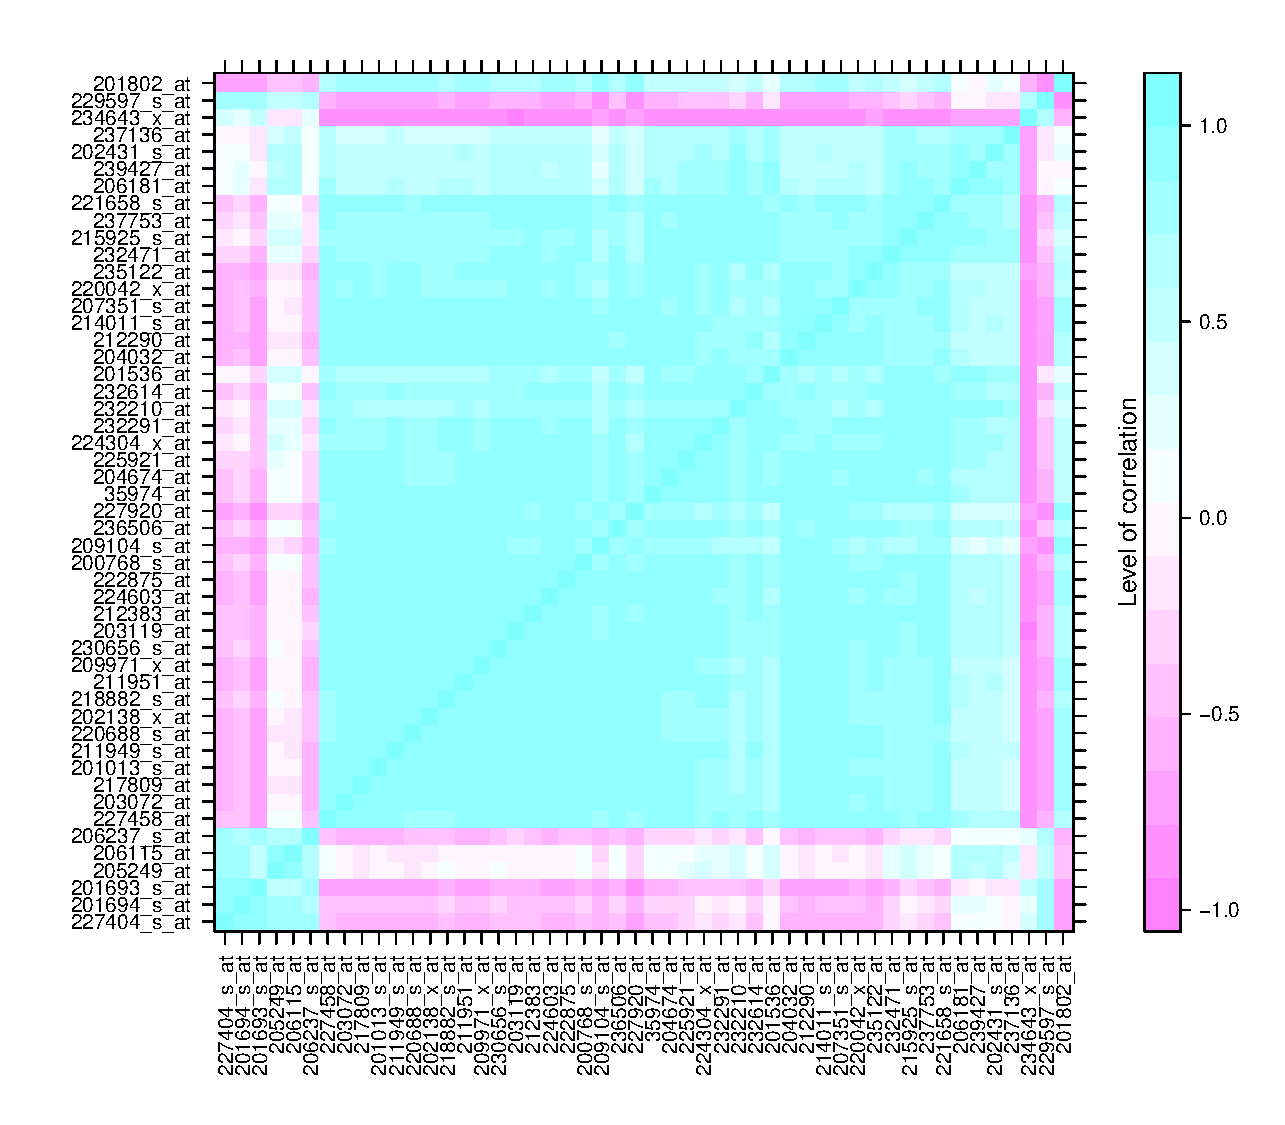
\includegraphics[clip=true,trim= 5mm 9mm 1mm 2mm]{Cascade-fig2.pdf}
\caption{Correlation between genes}\label{ind2}
\end{figure}
\restoregeometry



Note that a hierarchical clustering (function \texttt{agnes} of package \texttt{cluster}) is performed before plotting the result. This allows pointing out some structures, as correlated objects will be close in the graph. \\

If we want to select genes that are differentially expressed at specific time points we use the option \texttt{wanted.patterns}:


\begin{Schunk}
\begin{Sinput}
> #If we want to select genes that are differentially 
> #at time t60 or t90 :
> Selection<-geneSelection(x=micro_S,y=micro_US,tot.number=30,
   wanted.patterns=
   rbind(c(0,1,0,0),c(1,0,0,0),c(1,1,0,0)))
\end{Sinput}
\end{Schunk}

You may want forbid some patterns thanks to the \texttt{forbidden.patterns} option. \\

If we wish select genes that have a differential maximum of expression at a specific time point, we may use the \texttt{genePeakSelection} method. Basically, this function selects genes that are differentially expressed at desired time point, and which differential expression is significantly higher at this time point:

\begin{Schunk}
\begin{Sinput}
> Selection<-genePeakSelection(x=micro_S,y=micro_US,1,
   abs_val=FALSE,alpha_diff=0.01)
\end{Sinput}
\end{Schunk}


If there are more than two microarrays of interest, geneSelection may be used with a list of  microarrays as first argument, and a list specifying the contrast as a second argument:


\begin{itemize}
\item[First element:] ``condition", ``condition\&time" or ``pattern". The ``condition" specification is used when the overall goal is to compare two conditions. 
The ``condition\&time" specification is used when comparing two conditions at two precise time points.
The ``pattern" specification allows to choose at which time points selected a gene should be expressed or not. 
\item[Second element:] a vector of length 2, corresponding to the two conditions that should be compared. If a non-temporal dataset is used as control, it should be the first element of the micro\_array list and the option ``cont=TRUE" should be used. 
\item[Third element:] depends on the first element. 
This element is not needed if ``condition" has been specified. 
If ``condition\&time" has been specified, then this is a vector containing the time point at which the comparison should be done.
If ``pattern" has been specified, then this is a vector of 0 and 1 of length T, where T is the number of time points. 
Time points where differential expression is wanted are provided with 1. 
\end{itemize}


We can now compute an effective selection. As shown in Figure \ref{finalselec}, the early time points ($t_1=$60 and $t_2=$90) are correlated together and the later time points  ($t_3=$210 and $t_4=$390) are correlated together; this is a fact that is well known in the literature (\cite{yosef2011impulse}). \\

As an illustrating example, the following selection will be used for reverse-engineering:

\begin{Schunk}
\begin{Sinput}
> #Genes with differential expression at t1
> Selection1<-geneSelection(x=micro_S,y=micro_US,20,wanted.patterns= rbind(c(1,0,0,0)))
> #Genes with differential expression at t2
> Selection2<-geneSelection(x=micro_S,y=micro_US,20,wanted.patterns= rbind(c(0,1,0,0)))
> #Genes with differential expression at t3
> Selection3<-geneSelection(x=micro_S,y=micro_US,20,wanted.patterns= rbind(c(0,0,1,0)))
> #Genes with differential expression at t4
> Selection4<-geneSelection(x=micro_S,y=micro_US,20,wanted.patterns= rbind(c(0,0,0,1)))
> #Genes with global differential expression 
> Selection5<-geneSelection(x=micro_S,y=micro_US,20)
\end{Sinput}
\end{Schunk}

We then make the union between these different selections:

\begin{Schunk}
\begin{Sinput}
> Selection<-unionMicro(list(Selection1,Selection2,Selection3,Selection4,Selection5))
> print(Selection)
\end{Sinput}
\begin{Soutput}
This is a micro_array S4 class. It contains : 
 - (@microarray) a matrix of dimension  74 * 24 
          .... [gene expressions] 
 - (@name) a vector of length  74  .... [gene names] 
 - (@group) a vector of length  74  .... [groups for genes] 
 - (@start_time) a vector of length  74 
          .... [first differential expression for genes] 
 - (@time)a vector of length  4  .... [time points]
 - (@subject) an integer  .... [number of subject]
\end{Soutput}
\end{Schunk}

We use the \texttt{org.Hs.eg.db} Bioconductor database to match probesets with gene ID:


\begin{Schunk}
\begin{Sinput}
> library(org.Hs.eg.db)
> ff<-function(x){substr(x, 1, nchar(x)-3)}
> ff<-Vectorize(ff)
> #Here is the function to transform the probeset names to gene ID.
> 
> library("hgu133plus2.db")
> probe_to_id<-function(n){  
   x <- hgu133plus2SYMBOL
   mp<-mappedkeys(x)
   xx <- unlist(as.list(x[mp]))
   genes_all = xx[(n)]
   genes_all[is.na(genes_all)]<-"unknown"
   return(genes_all)
   }
> Selection@name<-probe_to_id(Selection@name)
> #Prints the correlation graphics Figure 4:
> summary(Selection,3)
\end{Sinput}
\end{Schunk}

\newgeometry{scale=0.85}
\begin{figure}
\centering
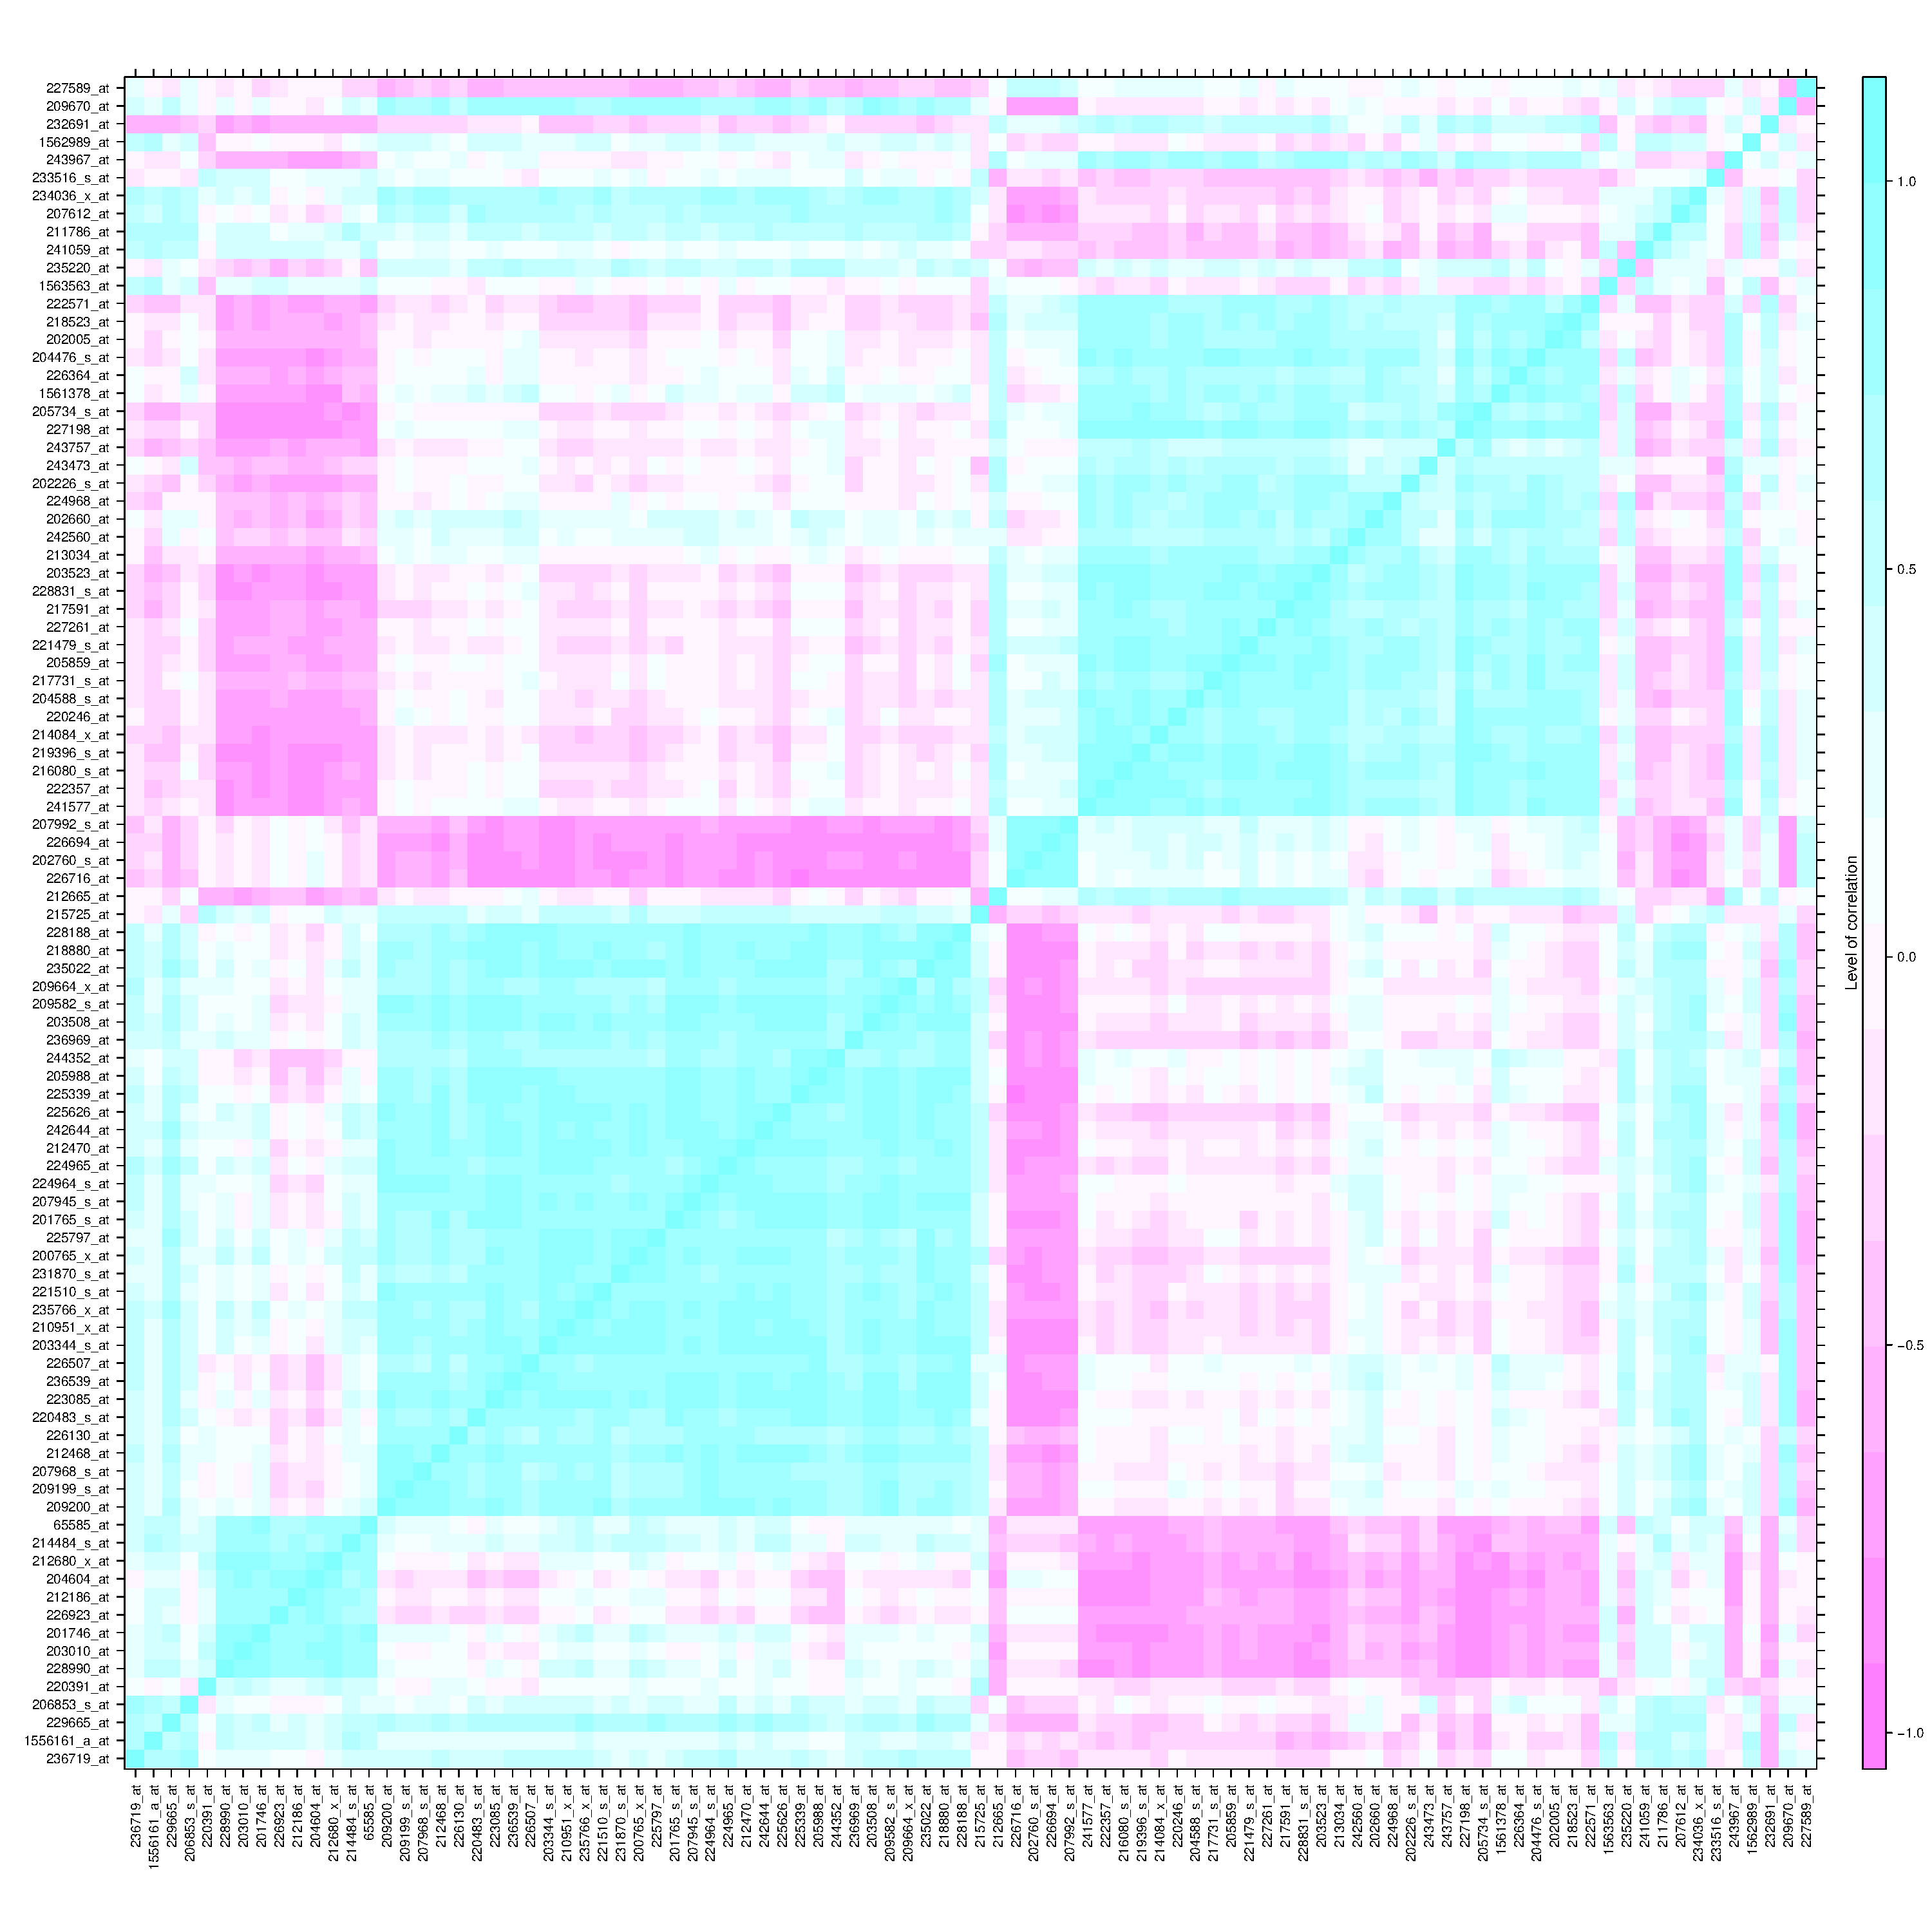
\includegraphics[width=17cm]{z.pdf}
\caption{Correlation structure of the final selection}
\label{finalselec}
\end{figure}
\restoregeometry


\section{Gene regulatory network reverse-engineering}
\subsection{Theoretical background}

Our gene regulatory network reverse-engineering method relies on a Lasso penalized estimation of a linear regression model (\cite{tib}). Before describing our model, we make some general reminders of the Lasso estimator.

\subsubsection{The Lasso estimate}

Suppose that we have data $(\boldsymbol{x_{i.}},y_i)_{i=1,\dotsb,N}$ where the $\boldsymbol{x_{i.}}=(x_{i1},\dotsb,x_{ip})^T$ are the predictors while the $y_i$ are the response. 
The linear regression model is:

\begin{equation}
 y_i= \sum_{j=1}^{p} {\beta}_j  x_{ij} + \eta_i,
\end{equation}

where $\eta_i$ is a noise following some probabilistic distribution.\\

Assume that the predictors are standardized and that the response is centered. The Lasso estimate is then given by:

\begin{equation}\label{lasso1}
\hat{\boldsymbol{\beta}}^L(\lambda)=\underset{{\boldsymbol{\beta}} \in \mathbb{R}^p}{\operatorname{argmin}} \left[ \sum_{i=1}^{N} \left(y_i- \sum_{j=1}^{p} {\beta}_j  x_{ij}\right)^2 +  \lambda \| \boldsymbol{\beta}\|_1\right],
\end{equation}

with $\lambda$ a non-negative scalar that determines the level of the constraints which is user-provided. We remark that:

\begin{itemize}
\item When $\lambda = 0$, $\hat{\boldsymbol{\beta}}^L$ is an ordinary least square estimation.
\item When $\lambda = +\infty$, we get $\hat{\boldsymbol{\beta}}^L = \boldsymbol{0}_p$.
\end{itemize}

The Lasso estimate for linear regression has two main advantages: 

\begin{enumerate}
\item it allows dealing with ill-posed problems where the number of observations is inferior to the number of variables,
\item it allows performing variable selection: for a proper choice of $\lambda$, $\hat{\boldsymbol{\beta}}^L(\lambda)$ will be parsimonious. \\
\end{enumerate}

The Lasso estimate for linear regression can also be written in the following form: 

\begin{equation}\label{lasso2}
\hat{\boldsymbol{\beta}}^L(\lambda)=\underset{{\boldsymbol{\beta}} \in \mathbb{R}^p ~~ \| \boldsymbol{\beta}\|_1 \leq \tilde{\lambda}}{\operatorname{argmin} } \left[ \sum_{i=1}^{N} \left(y_i- \sum_{j=1}^{p} {\beta}_j  x_{ij}\right)^2 \right].
\end{equation}

These two formulations (equation \eqref{lasso1} which is the penalized formulation and equation \eqref{lasso2} which is the constrained formulation) are equivalent in the sense that for each non negative $\lambda$ there is a non-negative  $\tilde{\lambda}$ leading to the same solution. \\

\subsubsection{Model for network reverse-engineering}

Suppose that we have selected $N$ genes across $T$ time points and for $P$ individuals; we note $x_{npt}$ the expression of gene $n$ for individual $p$ at time-point $t$. 
Since each gene will be considered exactly once as a response variable, our model is composed of $N$ linear regression models. 
As the action of a gene of another is not instantaneous, we define:

$$
\tilde{\boldsymbol{x}}_{np.} = 
\begin{pmatrix}
x_{np{t_2}} \\
\vdots \\
x_{np{t_T}}
\end{pmatrix}
\text{~~~and~~~}
\check{\boldsymbol{x}}_{np.} = 
\begin{pmatrix}
x_{np{t_1}} \\
\vdots \\
x_{np{t_{T-1}}}
\end{pmatrix},
$$

$$
\tilde{\boldsymbol{x}}_{n..} = 
\begin{pmatrix}
\tilde{\boldsymbol{x}}_{n1.}\\
\vdots \\
\tilde{\boldsymbol{x}}_{nP.}
\end{pmatrix}
\text{~~~and~~~}
\check{\boldsymbol{x}}_{n..} = 
\begin{pmatrix}
\check{\boldsymbol{x}}_{n1.} \\
\vdots \\
\check{\boldsymbol{x}}_{nP.}
\end{pmatrix}.
$$

We note that $\tilde{\boldsymbol{x}}_{np.}$ begins at time point $t_2$ and ends at time point $t_T$, 
while  $\check{\boldsymbol{x}}_{np.}$ begins at time point $t_1$ and ends at time point $t_{T-1}$. 
In the following, when gene $n$ is the response variable we will use $\tilde{\boldsymbol{x}}_{np.}$, 
and $\check{\boldsymbol{x}}_{np.}$ when gene $n$ is a predictor variable. \\

We further assume that each gene has been assigned in one of the $T$ time-cluster (one cluster for each time).\\


We have previously proposed (\cite{vallat2013reverse}) the follwing linear regression model:

$$
\tilde{\boldsymbol{x}}_{n..} = \sum_{n'=1}^{N} \boldsymbol{F}_{m(n')m(n)} \omega_{n'n} \check{\boldsymbol{x}}_{n'..} +\boldsymbol{\varepsilon}_{n},
$$

where:   \\

\begin{itemize}
\item $m(\bullet)$ is the function that maps a gene to its time-cluster,
\item $\boldsymbol{F}_{m(n')m(n)} $ is a $T-1$ square matrix that describes the action of genes,
\item $\omega_{n'n}$ is the strength of the connection from gene $i$ toward gene $j$,
\item $\boldsymbol{\varepsilon}_{n}$ is noise vector of length $T-1$. \\
\end{itemize} 

We choose to use a Lasso estimate for our linear regression model:


\begin{equation*} 
(\hat{\boldsymbol{\omega}},\hat{\boldsymbol{F}})=\underset{\begin{subarray}{c}
\omega_{n'n} \in \mathbb{R},~1\leq n',n\leq N\\
\boldsymbol{F}_{ab} \in \mathcal{M}_{T-1}(\mathbb{R}), 1\leq a,b \leq T
  \end{subarray} }{\operatorname{argmin} }\left[ \sum_{n=1}^{N}\left(\tilde{\boldsymbol{x}}_{n..} - \sum_{n'=1}^{N} \boldsymbol{F}_{m(n')m(n)} \omega_{n'n} \check{\boldsymbol{x}}_{n'..}\right)^2\right],
\end{equation*}

with the constraint: 

$$
\forall n = 1,...,N, ~~~ \sum_{n'=1}^N \omega_{n'n} \leq {\lambda_n}.
$$




So, $\tilde{\boldsymbol{x}}_{n..}$ is the regulated gene and $\boldsymbol{x}_{n'..}, n'=1,\dotsb,N$ are the regulators.  Notice that matrix $  F_{m(n')m(n)}$ permits to the link between genes $n'$ and $n$ to evolve across time. To enforce temporal causality we need the two following time constraints:

\begin{enumerate}
\item $m(n') \geq m(n) \Rightarrow \boldsymbol{F}_{m(n')m(n)} = 0$: this ensures that a gene with temporal cluster $t_k$ can influence a gene with temporal cluster $t_{k'}$ if and only if $k<k'$,
\item the matrices $ \boldsymbol{F}$ are lower triangular matrices: this ensures that the expression of a gene at time  $t_k$ can influence another gene at time $t_{k'}$ if and only if $k<k'$.
\end{enumerate}

Sub-diagonals and the diagonal of matrices $F$ are supposed to be invariant (\cite{vallat2013reverse}). Consequently, interactions depend only on time index differences rather than absolute time index. \\



We solve this problem with a coordinate ascent approach, by iteratively supposing the $ \boldsymbol{F}$ matrices or the $\omega_{n'n}$ matrices known. The result of the optimization is a connectivity network described by the nonzero elements of  $\hat{\omega}_{n'n}(obs)$ combined with a set of cluster-dependent interaction models described by the set $   \hat{\boldsymbol{F}}_{m(n')m(n)}(obs)$.\\

However, if clusters are sufficiently homogeneous, inference of matrices \linebreak 
$ \boldsymbol{F}_{m(n')m(n)}$ doesn't depend on which genes are active (\textit{i.e.} which $\omega_{n'n} \neq 0$). That's why a non iterative algorithm is proposed in which estimation of   of matrices $F_{m(i)m(j)}$  precedes estimation of matrix $\boldsymbol{\Omega}$.\\

To get a more robust result, at each step, the estimation of matrices \linebreak  $ \boldsymbol{F}_{m(n')m(n)}$ is done several times throughout cross-validation. Furthermore, to avoid computational issues, the new solution is chosen by a linear combination between the old and the new solution. 



\subsection{Performing the reverse-engineering algorithm}

To perform this algorithm on our data:

\begin{Schunk}
\begin{Sinput}
> network<-inference(Selection)
\end{Sinput}
\begin{Soutput}
We are at step :  1
The convergence of the network is (L1 norm) : 0.01096
We are at step :  2
The convergence of the network is (L1 norm) : 0.00302
We are at step :  3
The convergence of the network is (L1 norm) : 0.00217
We are at step :  4
The convergence of the network is (L1 norm) : 0.00177
We are at step :  5
The convergence of the network is (L1 norm) : 0.00146
We are at step :  6
The convergence of the network is (L1 norm) : 0.00111
We are at step :  7
The convergence of the network is (L1 norm) : 0.00089
\end{Soutput}
\end{Schunk}



We can plot a representation of $F$ matrices (Figure \ref{F1}) and the resulting network (Figure \ref{net1}) by simply using the \texttt{plot} method:
\begin{Schunk}
\begin{Sinput}
> plot(network,choice="F")
> plot(network,choice="network",gr=Selection@group,label_v=Selection@name)
\end{Sinput}
\end{Schunk}

Note that all network plots are computed using the Igraph R package (\cite{igraph}). \\ 



\begin{figure}
\centering
\includegraphics[width=10cm]{Cascade-fig3}
\caption{The F matrices ; for each matrix, the first bar plot corresponds to the coefficient of the diagonal, the second to the first sub-diagonal...}\label{F1}
\end{figure}

\newgeometry{scale=0.85}
\begin{figure}
\centering
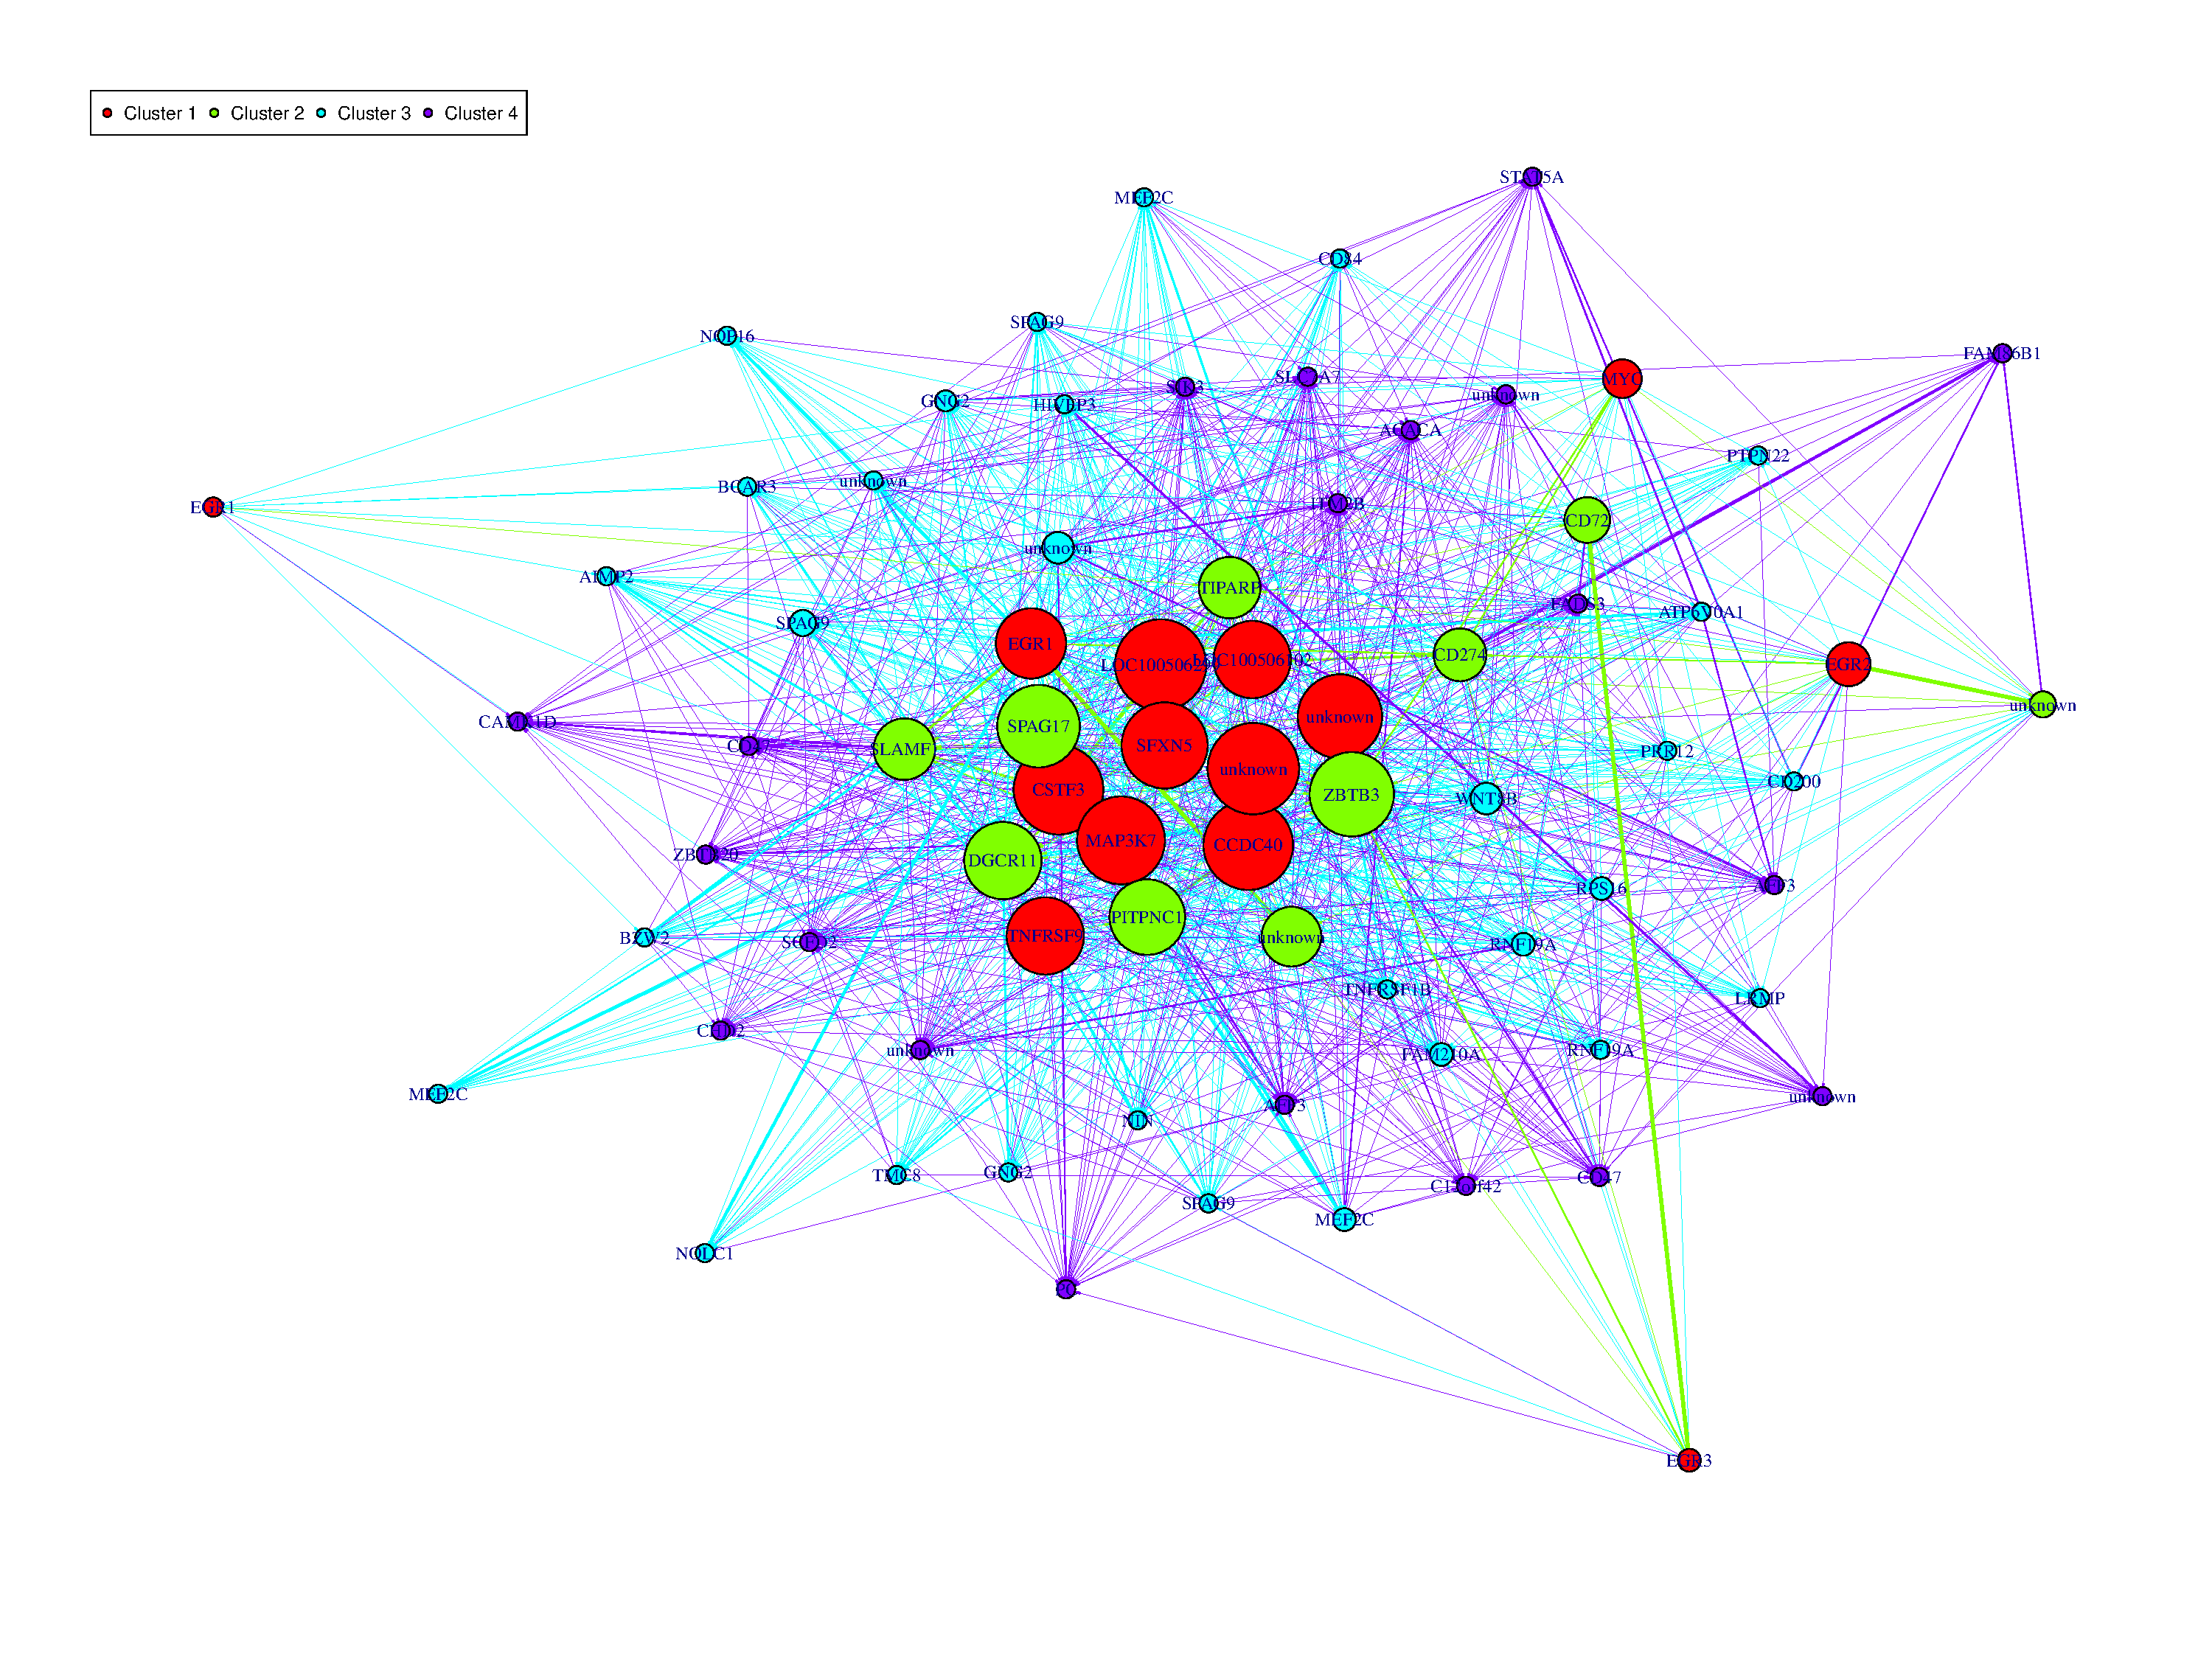
\includegraphics[clip=true,trim= 2cm 1cm 1mm 1cm,angle=90,width=18cm]{Cascade-fig4}
\caption{The resulting network with all edges}\label{net1}
\end{figure}
\restoregeometry




The number of edges in the network makes the message difficult to interpret ; and as we will see in the next section, results in term of predictive positive value and F-score can be improved when choosing a right cutoff level. Using the \texttt{nv} option, we will choose a cutoff under which the regression coefficient estimates ($\hat{\omega_{ij}}(obs)$) are set to $0$. In Figure \ref{net2} a cutoff of 0.2 is chosen. 

\subsection{Choosing the best cutoff for edge minimal strength}

The difficulty is now to choose the best cutoff. As a starting point, we propose method \texttt{evolution}, that allows the user to see, in a html page, the evolution of the network when the cutoff is growing up. When the \texttt{fix} option is set to \texttt{FASLE}, at each step the position of the genes are re-calculated. 

\begin{Schunk}
\begin{Sinput}
> evolution(network,seq(0,0.4,by=0.01),gr=Selection@group,fix=TRUE,label_v=Selection@name)
> evolution(network,seq(0,0.4,by=0.01),gr=Selection@group,fix=FALSE,label_v=Selection@name)
\end{Sinput}
\end{Schunk}

To see the result of these functions, go to :

\begin{itemize}
\item \url{http://www-irma.u-strasbg.fr/~njung/evolution_fix_true/evol.html} : here the \texttt{fix} option is set to \texttt{TRUE}.
\item \url{http://www-irma.u-strasbg.fr/~njung/evolution_fix_false/evol.html}: here the \texttt{fix} option is set to \texttt{FALSE}.
\end{itemize}

As it is mostly accepted, gene regulatory networks are supposed to be scale-free (\cite{jeong2000large}). 
The notion of scale freeness in networks relies on the probability distribution of the number of outgoing edges. 
A network is called scale free when this distribution is a power law distribution (\cite{clauset2009power}). 
As this family of law is large, it is difficult to test such an hypothesis. 
We used the test proposed by Clauset \textit{et al.}(\cite{clauset2009power}):


%chunk 26
\begin{Schunk}
\begin{Sinput}
> evol_cutoff<-cutoff(network)
> nv<-0.11
\end{Sinput}
\end{Schunk}


We plot here the smooth interpolation rather than the exact values, as our interest relies mostly on the trend (Figure \ref{eve}). We propose a choice of cutoff that relies on two criteria: 

\begin{itemize}
\item the p-value should be greater than 0.10: in this case, the scale-freeness of the network is reliable (\cite{clauset2009power}).
\item we determined by simulation the best area of choice (on the plot (Figure \ref{eve})). \\
\end{itemize}

Based on these two criteria, we choose a cutoff of $nv=0.11$. 




\newgeometry{scale=0.85}
\begin{figure}
\centering
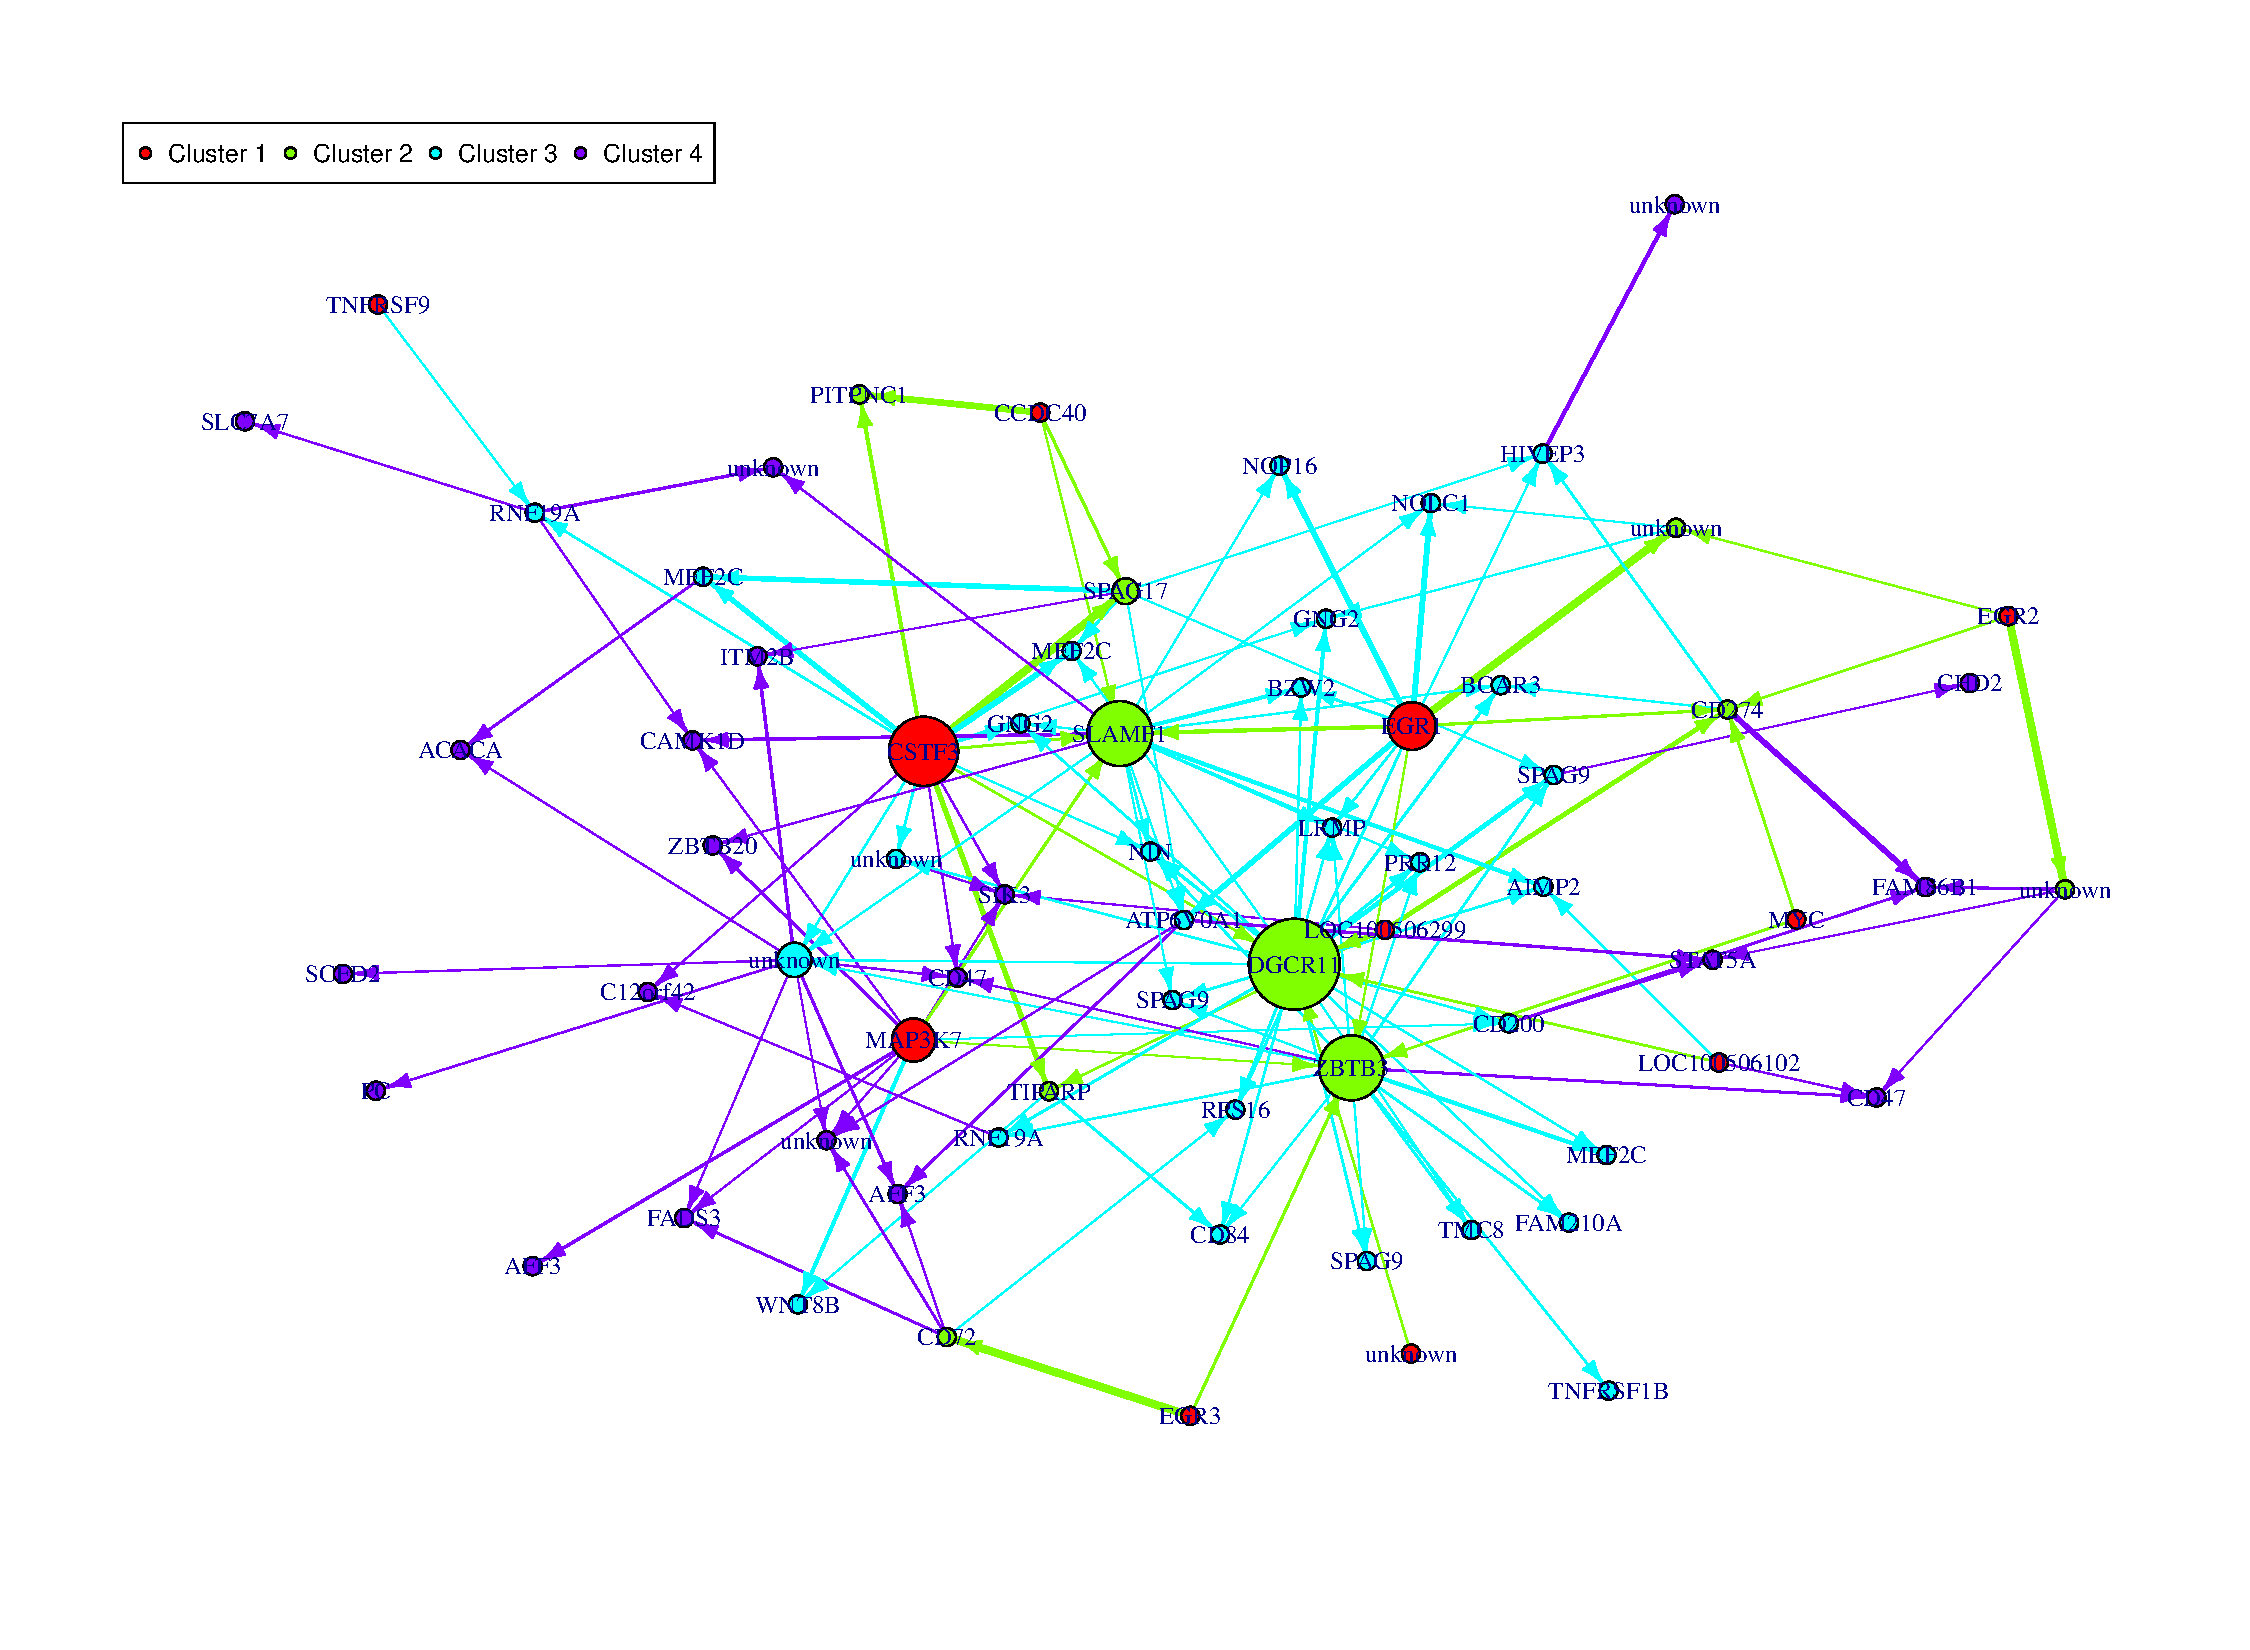
\includegraphics[clip=true,trim= 2.05cm 3cm 2cm 2cm]{Cascade-fig5}
\caption{The resulting network with a cutoff of 0.11}\label{net2}
\includegraphics[width=10cm]{Cascade-fig6}
\caption{Evolution of scale-freeness of the network in function of the cutoff. The p-value corresponds to the adequacy of the data to a power law distribution. }\label{eve}
\end{figure}
\restoregeometry

\subsection{Analyzing the network}

One may want to know which genes are important in the network. In our representation, the bigger the vertex the larger the number of outgoing edges. Indeed, genes with many outgoing edges, the hubs, are important in the network. 
But genes controlling these hubs should be considered with attention. The \texttt{analyze\_network} method allows computing different indicators:

\begin{itemize}
\item betweenness : it is a measure of the node centrality. It is calculated, for node $n$, by the following formula: 
$$
\sum_{s\neq t \neq n}\frac{\sigma_{st}(n)}{\sigma_{st}}
$$

where $\sigma_{st}$ is the number of shortest ways between $s$ and $t$, and $\sigma_{st}(n)$ is the number of shortest ways between $s$ and $t$ passing by $n$ ;
\item degree : the number of outgoing edges ;
\item output : the sum of weights of outgoing genes ;
\item closeness : it is a measure of the distance (in terms of shortest path) of a gene to others.
\end{itemize}

As our network is weighted we used specific measures developed by Opsahl (\cite{bla}).
 
\begin{Schunk}
\begin{Sinput}
> analyze<-analyze_network(network,nv,Selection@name)
> head(analyze)
\end{Sinput}
\begin{Soutput}
          node betweenness degree    output closeness
1 LOC100506299           0      4 0.9480871 21.733638
2       CCDC40           0      3 0.8884602 14.957508
3      unknown           0      1 0.1749376 13.272288
4 LOC100506102           0      3 0.5159878 15.045094
5      TNFRSF9           0      1 0.1243596  1.630903
6        CSTF3           0     16 3.9603909 34.135176
\end{Soutput}
\end{Schunk}

Note that one can plot the network and modulate the size of the vertex following one of this measure, using the \texttt{weight.node} option. \\

Using again the package \texttt{animation}, we can see how the signal spreads in the network by turning to \texttt{TRUE} the option \texttt{ani}:

\begin{Schunk}
\begin{Sinput}
> plot(network,nv=nv,gr=Selection@group,ani=TRUE,
   ,label_v=Selection@name,
   edge.arrow.size=0.9,edge.thickness=1.5)
\end{Sinput}
\end{Schunk}

Result is available at \url{http://www-irma.u-strasbg.fr/~njung/network_spread/spread.html}. \\


The method \texttt{plot} has basically two steps: 

\begin{enumerate}
\item it calculates the position of the vertex,
\item  it plots the graph.
\end{enumerate} 

In some case, it is interesting to produce two plots of a same network without changing vertex positions. Here is a way to do that, using the \texttt{ini} option of method plot:

\begin{Schunk}
\begin{Sinput}
> P<-position(network,nv=nv)
> #plotting the network with the given position
> plot(network,nv=nv,gr=Selection@group,ini=P,label_v=Selection@name)
\end{Sinput}
\end{Schunk}

 
However, we didn't develop all possibilities of the \texttt{plot} option ; for more possibilities, please refer to the manual:

\begin{Schunk}
\begin{Sinput}
> vignette("Cascade-manual")
\end{Sinput}
\end{Schunk}



\section{Prediction of gene expression modulations after a knock-out experiment}

Once the network has been reverse-engineered, we want to know the impact of an experimental perturbation in this network. For example, what would happen if expression of EGR1 is knocked-out ?

\begin{Schunk}
\begin{Sinput}
> EGR1<-which(Selection@name %in% "EGR1")
\end{Sinput}
\end{Schunk}

First the \texttt{geneNeighborhood} method allows determining which are the neighborhood of EGR1 (see Figure \ref{neig}). \\

\begin{Schunk}
\begin{Sinput}
> geneNeighborhood(network,targets=EGR1,nv=nv,ini=P,
   label_v=Selection@name)
> #label.hub: only hubs vertex should have a name
> #label_v: name of the vertex
\end{Sinput}
\end{Schunk}


We  predict gene expression modulations within the network if EGR1 is experimentaly knocked-out. 

%chunk 34
\begin{Schunk}
\begin{Sinput}
> prediction_ko5<-predict(Selection,network,nv=nv,targets= EGR1)
\end{Sinput}
\end{Schunk}

Then we plot the results (Figure \ref{pred}): 
\begin{Schunk}
\begin{Sinput}
> #We plot the results.
> #Here for example we see changes at time point t2:
> plot(prediction_ko5,time=2,ini=P,label_v=Selection@name)
\end{Sinput}
\end{Schunk}


\begin{figure}
\centering
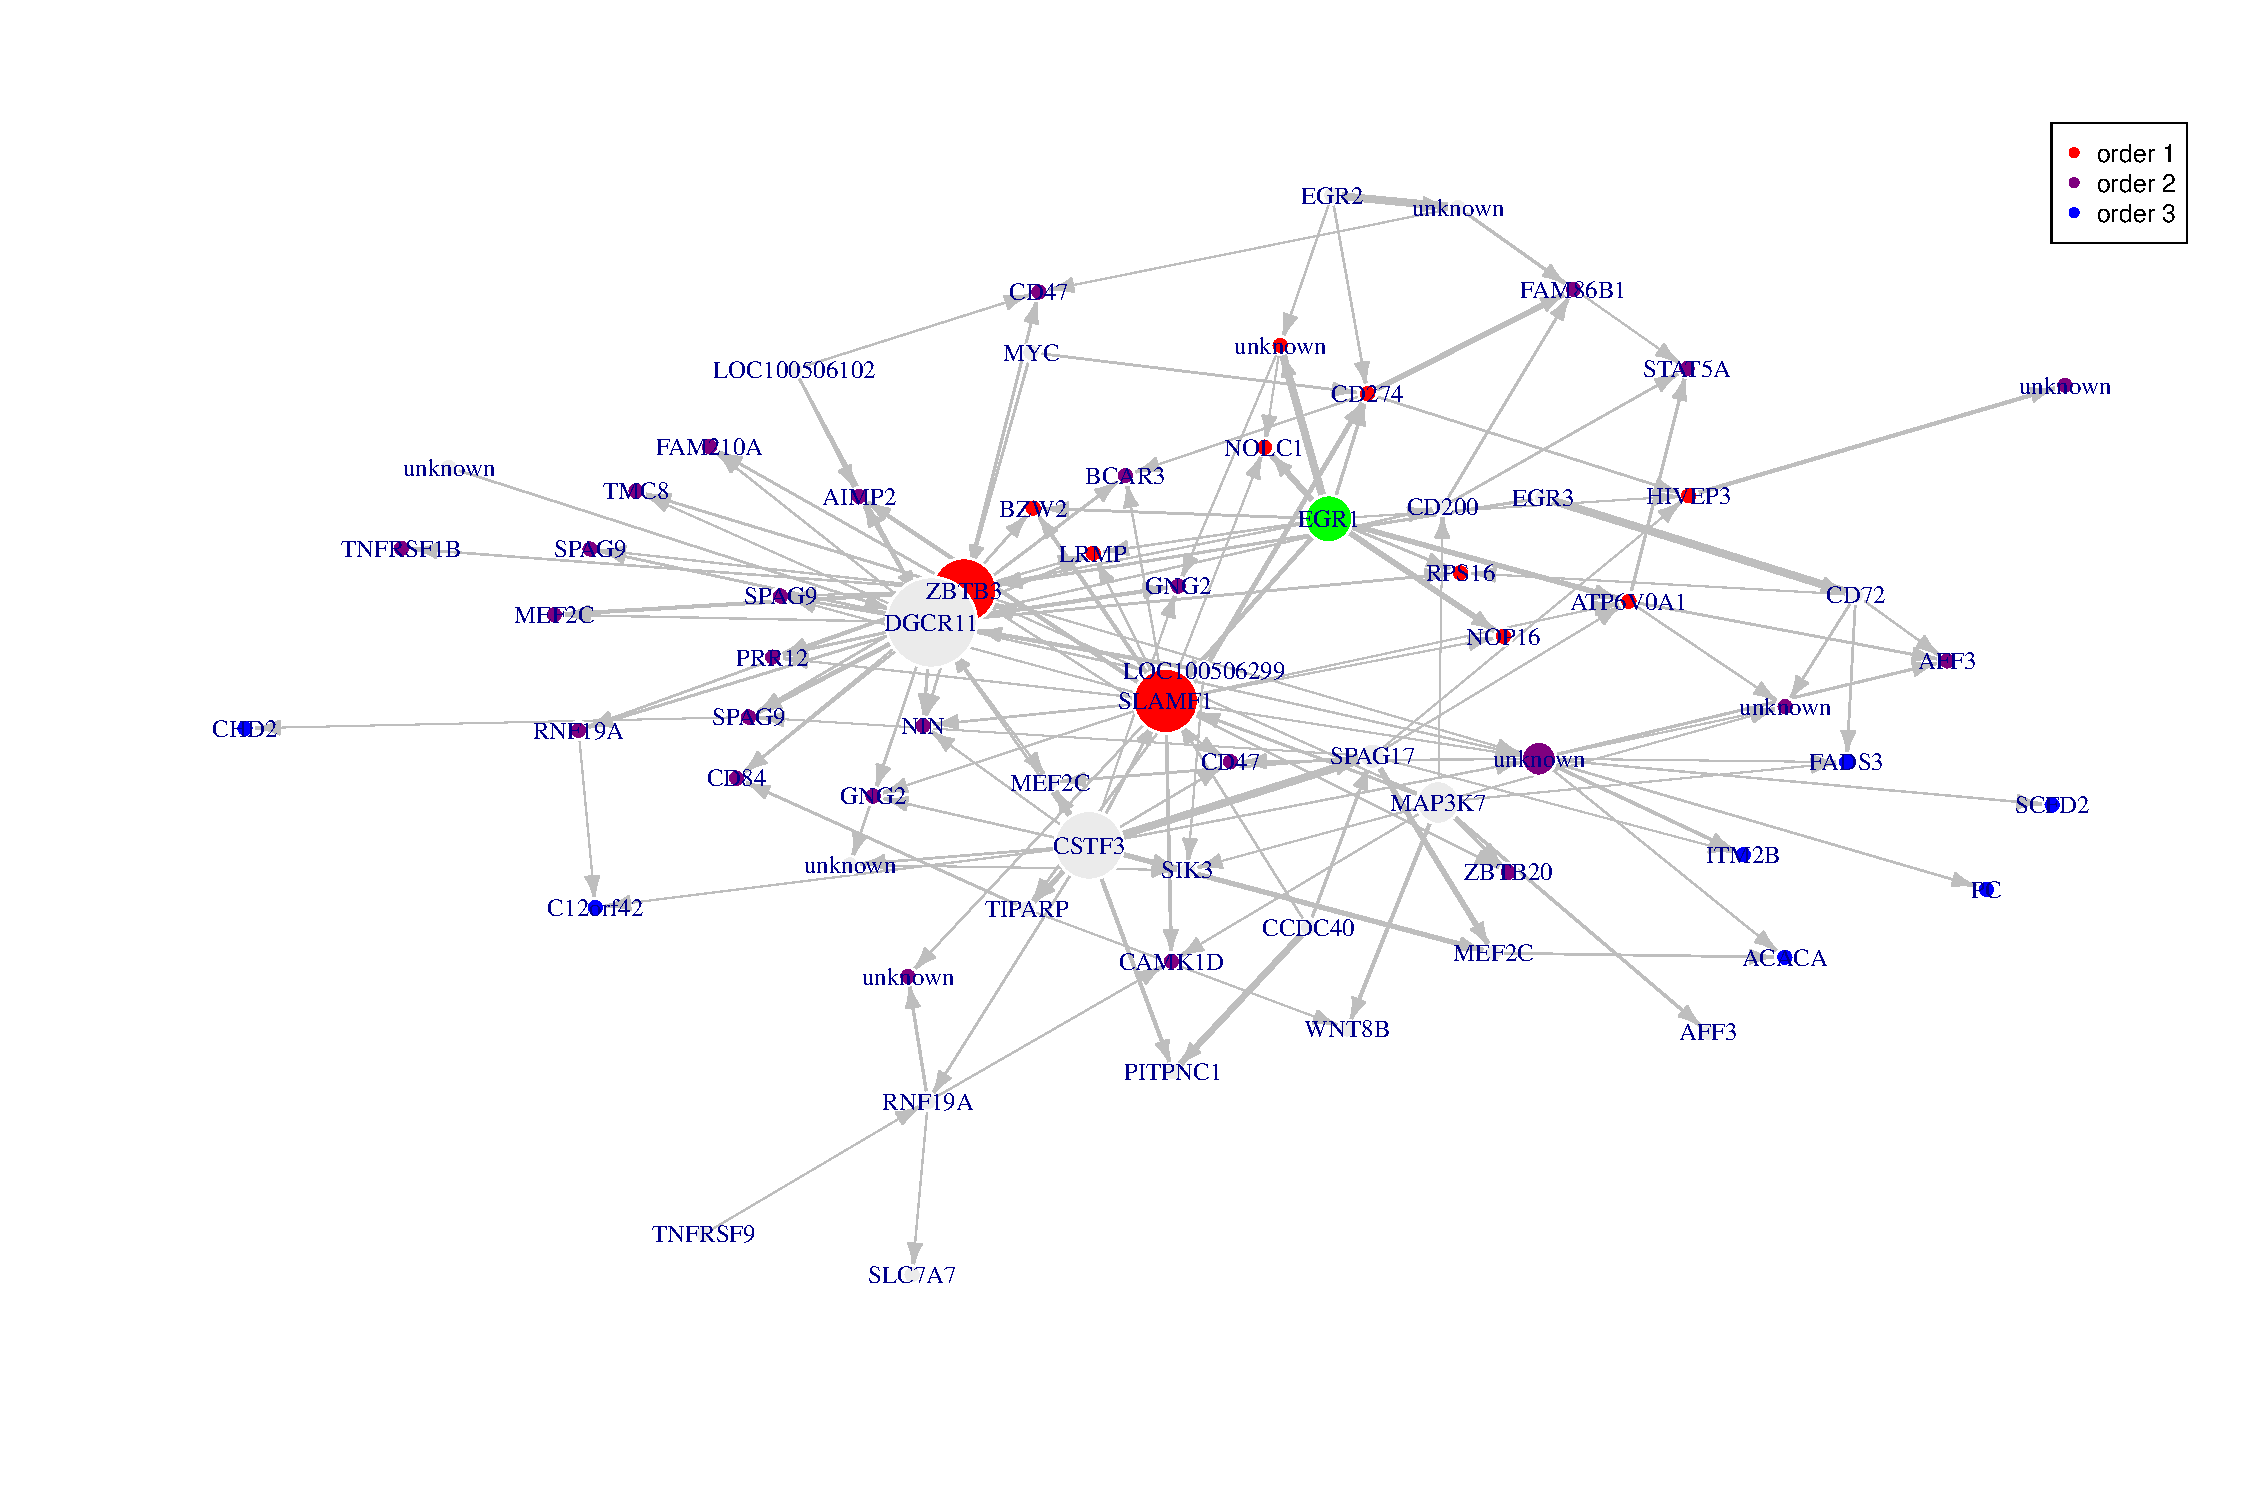
\includegraphics[clip=true,trim= 2cm 3cm 1mm 1cm,angle=0,width=17cm]{Cascade-fig7}
\caption{Neighborhood of gene EGR1} \label{neig}
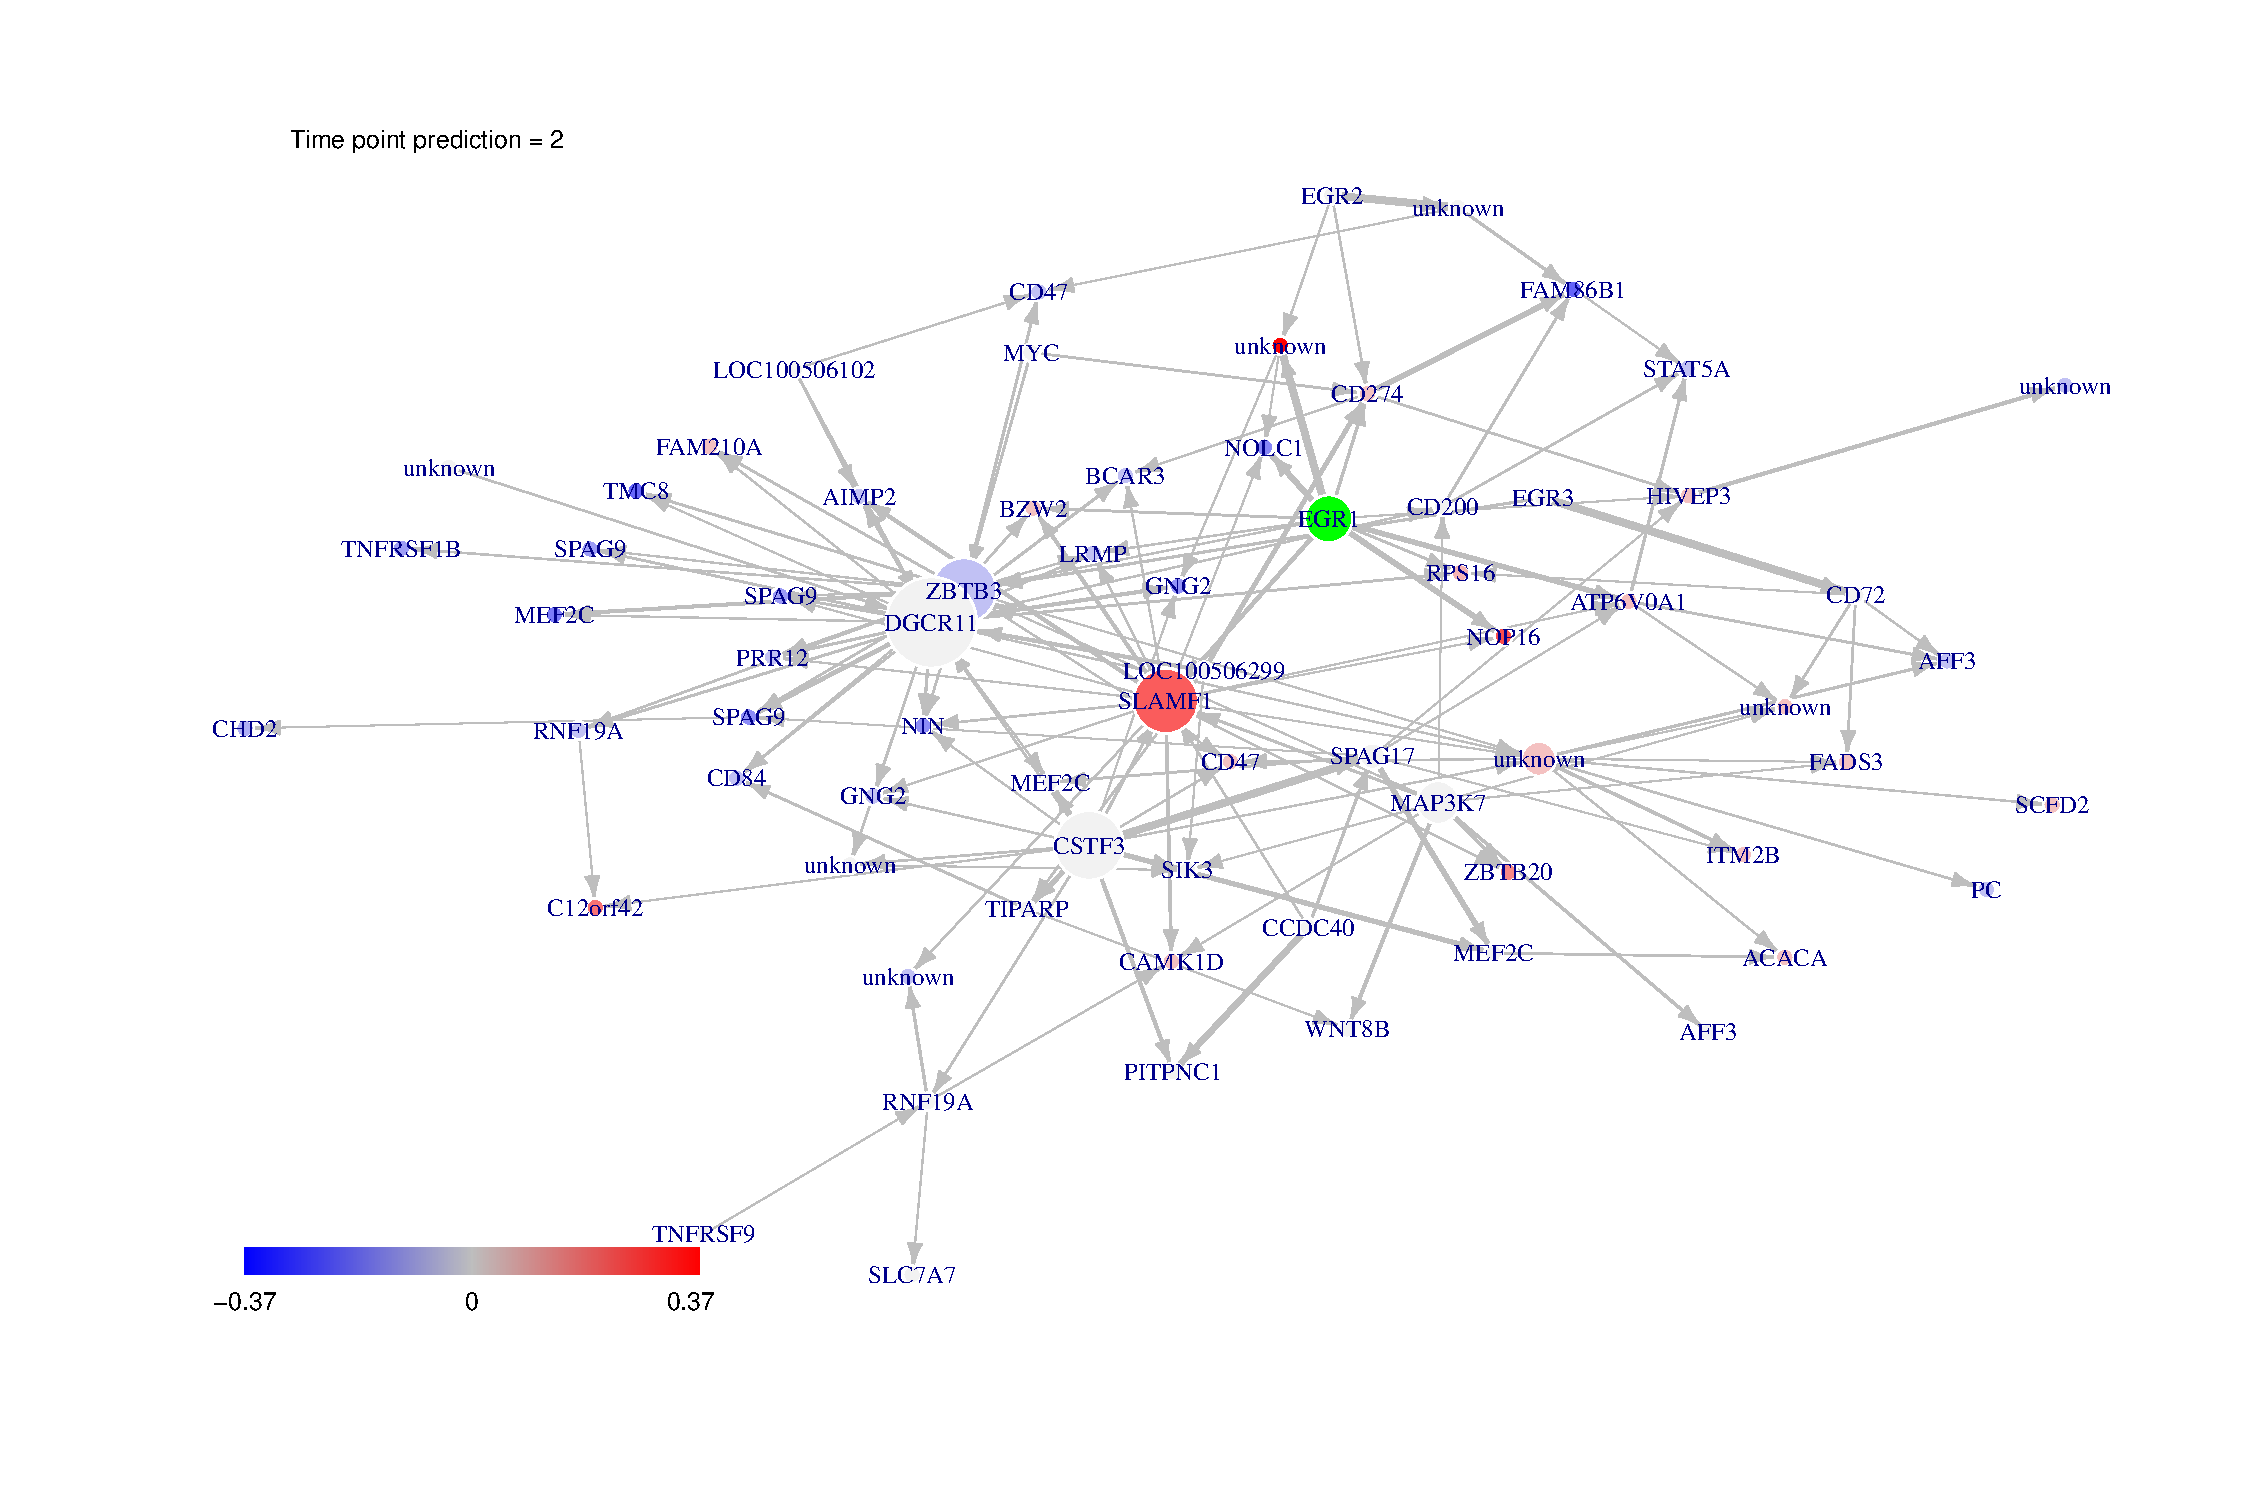
\includegraphics[clip=true,trim= 2cm 3cm 1mm 1cm,angle=0,width=17cm]{Cascade-fig8}
\caption{Perturbation modulation at time point 2 of the network consecutively to the knock-out of EGR1.} \label{pred}
\end{figure}
    

        

\section{Simulation}

To simulate gene expressions based on a gene regulatory network, we first have to generate the network. Here, we implemented an algorithm that is inspired by the \textit{preferential attachment} from Barab\'asi (\cite{barabasi2002emergence,jeong2007measuring}). We adapted this algorithm in our case of temporal cascade networks. \\

We then use our linear model to make some simulations, using Laplace laws to initiate the algorithm.  


\begin{Schunk}
\begin{Sinput}
> #We set the seed to make the results reproducible 
> set.seed(1)
> #We create a random scale free network
> Net<-network_random(
   	nb=100,
   	time_label=rep(1:4,each=25),
   	exp=1,
   	init=1,
   	regul=round(rexp(100,1))+1,
   	min_expr=0.1,
   	max_expr=2,
   	casc.level=0.4
   	)
> #We change F matrices
> T<-4 
> F<-array(0,c(T-1,T-1,T*(T-1)/2))
> for(i in 1:(T*(T-1)/2)){diag(F[,,i])<-1}
> F[,,2]<-F[,,2]*0.2
> F[2,1,2]<-1
> F[3,2,2]<-1
> F[,,4]<-F[,,2]*0.3
> F[3,1,4]<-1
> F[,,5]<-F[,,2]
> Net@F<-F
> #We simulate gene expression according to the network Net
> M<-gene_expr_simulation(
   	network=Net,
   	time_label=rep(1:4,each=25),
   	subject=5,
   	level_peak=200)
\end{Sinput}
\end{Schunk}


\begin{Schunk}
\begin{Sinput}
> #We infer the new network
> Net_inf<-inference(M)
\end{Sinput}
\end{Schunk}

\begin{Schunk}
\begin{Sinput}
> #Comparing true and inferred networks
> F_score<-rep(0,200)
> #Here are the cutoff level tested
> test.seq<-seq(0,max(abs(Net_inf@network*0.9)),length.out=200)
> u<-0
> for(i in test.seq){
   	u<-u+1
   	F_score[u]<-compare(Net,Net_inf,i)[3]
   }
\end{Sinput}
\end{Schunk}


\begin{Schunk}
\begin{Sinput}
> #Choosing the cutoff
> cut.seq<-cutoff(Net_inf)
> plot(cut.seq$sequence,cut.seq$p.value.inter)
\end{Sinput}
\end{Schunk}


Figure \ref{pred21} shows the evolution of the p-value of the scale-freeness test while 
Figure \ref{pred23} shows the corresponding evolution of the F-score. As shown, choosing the 
best cut-off allows a dramatic increase of the cut-off. \\

Figure \ref{pred22} show the evolution of the F-score when the number of individuals increase. 

\newpage






\begin{figure}
\centering
\includegraphics[angle=0,width=10cm]{Cascade-042}
\caption{Evolution of the scale-freeness of the network in function of the cutoff} \label{pred21}
\includegraphics[clip=true,width=10cm]{Cascade-fig10}
\caption{Evolution of F-score in function of the cutoff} \label{pred23}
\end{figure}



\begin{figure}
\centering
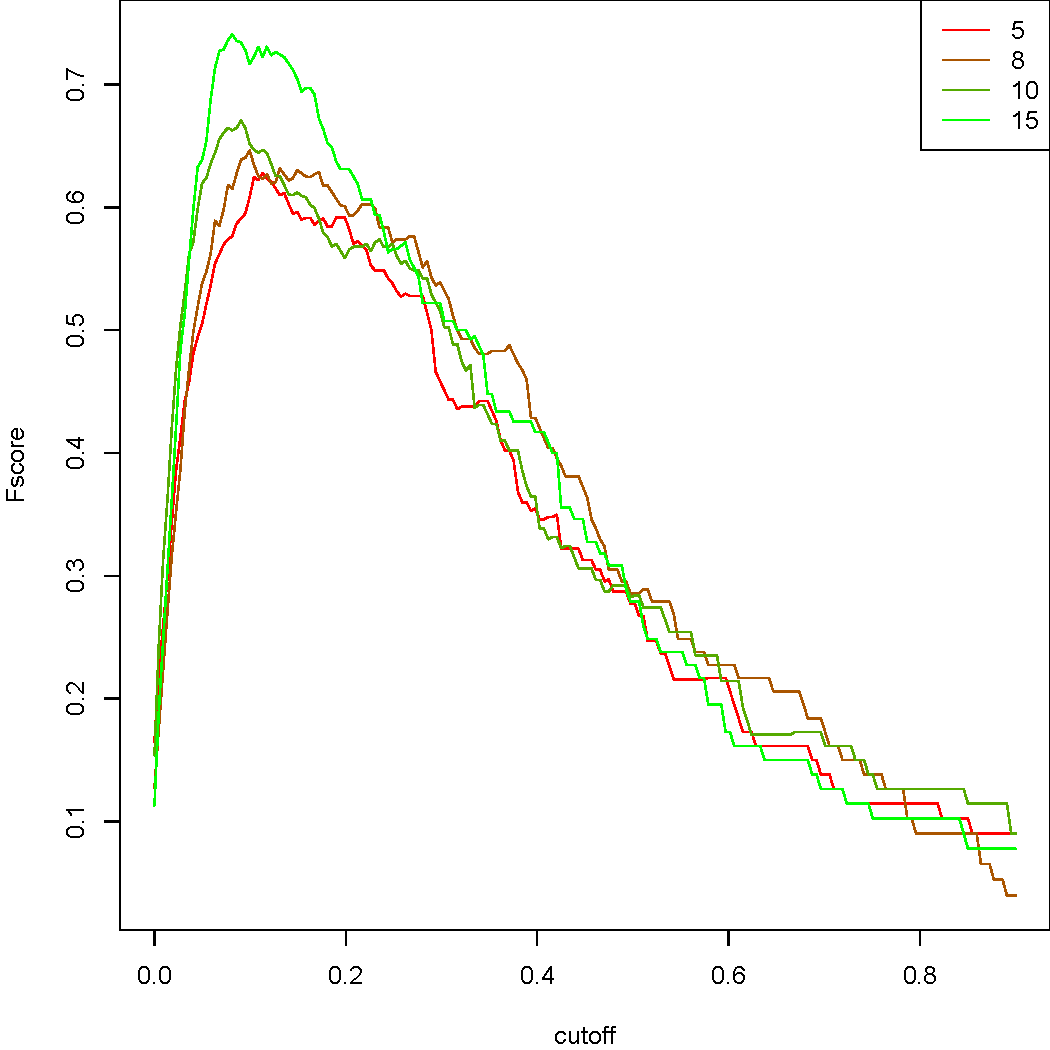
\includegraphics{subject_evol}
\caption{Evolution of F-score in function of the cutoff and the number of subject in the study} \label{pred22}
\end{figure}

\newpage
\clearpage
\bibliographystyle{apalike}
\bibliography{vignette} 
\end{document}
